
%%% Local Variables: 
%%% mode: latex
%%% TeX-master: t
%%% End: 

\section{Introduction}

The virtual object layer is an abstraction layer in the HDF5 library that intercepts all API calls that could potentially access objects in an HDF5 container and forwards those calls to a VOL connector, which implements the storage. The user or application gets the benefit of using the familiar and widely-used HDF5 data model and API, but can map the physical storage of the HDF5 file and objects to storage that better meets the application's data needs.

\subsection*{The VOL Abstraction Layer}

The VOL lies just under the public API. When a storage-oriented public API call is made, the library performs a few sanity checks on the input parameters and then immediately invokes a VOL callback, which resolves to an implementation in the VOL connector that was selected when opening or creating the file. The VOL connector then performs whatever operations are needed before control returns to the library, where any final library operations such as assigning IDs for newly created/opened datasets are performed before returning. This means that, for calls that utilize the VOL, all of the functionality is deferred to the VOL connector and the HDF5 library does very little work. An important consideration of this is that most of the HDF5 caching layers (metadata and chunk caches, page buffering, etc.) will not be available as those are implemented in the HDF5 native VOL connector and cannot be easily reused by external connectors.

\begin{figure}[h]
\caption {The VOL Architecture}
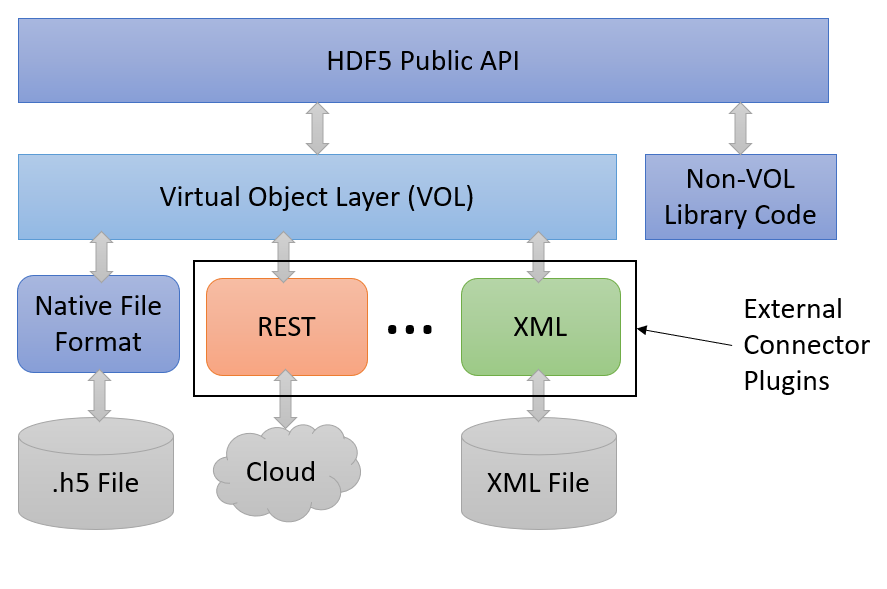
\includegraphics[width=\textwidth]{vol_architecture.png}
\end{figure}

Not all public HDF5 API calls pass through the VOL. Only calls which require manipulating storage go through the VOL and require a VOL connector author to implement the appropriate callback. Dataspace, property list, error stack, etc. calls have nothing to do with storage manipulation or querying and do not use the VOL. This may be confusing when it comes to property list calls, since many of those calls set properties for storage. Property lists are just collections of key-value pairs, though, so the VOL is not involved with setting or getting any properties.

Another thing to keep in mind is that not every VOL connector will implement the full HDF5 public API. In some cases, a particular feature like variable-length types may not have been developed yet or may not have an equivalent in the target storage system. Also, many HDF5 public API calls are specific to the native HDF5 file format and are unlikely to have any use in other VOL connectors. A feature/capabilities flag scheme is being developed to help navigate this.

For more information about which calls go through the VOL and the mechanism by which this is implemented, see the connector author and library internals documentation.

\subsection*{VOL Connectors}

An external VOL connector is normally implemented as a dynamically loaded plugin. In order to be used by an application, they must be discoverable and loadable via path settings, etc. These plugins are loaded at runtime via the same HDF5 plugin scheme used for filters. A VOL connector for a file is set in the file access property list (FAPL) used to open it, either via H5Pset\_vol() or a connector-specific API call provided by the connector author.

Many VOL connectors (at various stages of construction) can be found here:

\quad \quad https://bitbucket.hdfgroup.org/projects/HDF5VOL

Not every connector in this collection is actively maintained by The HDF Group. It simply serves as a single location where important VOL connectors can be found. See the documentation in a connector's repository to determine its development status and the parties responsible for it. The collection also includes a VOL template that contains build scripts (Autotools and CMake) and an empty VOL connector "shell" which can be copied and used as a starting point for building new connectors. See the VOL Connector Author Guide for more information on this.

The native VOL connector is a special case. It is currently implemented as a built-in part of the HDF5 library and cannot be unloaded, nor can its ID be closed.


\section{Quickstart}

\subsection*{Read The Documentation For The New VOL Connector}

Many VOL connectors will require specific setup and configuration of both the application and the storage. Specific permissions may have to be set, configuration files constructed, and connector-specific setup calls may need to be invoked in the application. In many cases, converting software to use a new VOL connector will be more than just a straightforward drop-in replacement done by specifying a name in the VOL plugin environment variable.

\subsection*{Use A VOL-Enabled HDF5 Library}

The virtual object layer was introduced in HDF5 1.12.0, so you will need that version or later to use it. The particular configuration of the library (serial vs parallel, thread-safe, debug vs production/release) does not matter. The VOL is a fundamental part of the library and cannot be disabled, so any build will do.

On Windows, it's probably best to use the same debug vs release configuration for the application and all libraries in order to avoid C runtime (CRT) issues. On pre-2015 versions of Visual Studio, you'll probably also want to stick to the same Visual Studio version (and thus same CRT version) as well.

When working with a debug HDF5 library, it's probably also wise to build with the "memory sanity checking" feature disabled to avoid accidentally clobbering our memory tracking infrastructure when dealing with buffers obtained from the HDF5 library.

\subsection*{Make Sure The VOL Connector Is In The Search Path}

The default location for all HDF5 plugins is set at configure time when building the HDF5 library. This is true for both CMake and the Autotools.

\textbf{Default locations:}

\begin{tabular}{ l l }
    POSIX systems: &  {\tt /usr/local/hdf5/lib/plugin} \\
     & \\
    Windows: & {\tt \%ALLUSERSPROFILE\%/hdf5/lib/plugin}
\end{tabular}

These default locations can be overridden by setting the {\tt HDF5\_PLUGIN\_PATH} environment variable. There are also public {\tt H5PL} API calls which can be used to add, modify, and remove search paths. The library will only look for plugins in the specified plugin paths. By default, it will NOT find plugins that are simply located in the same directory as the executable.

\subsection*{Update Your Code To Load And Use A VOL Connector}

How this is done depends on the VOL connector, which may have special API calls for setup or require appropriate configuration files, but the most generic way to modify a program to use a specific VOL connector would be to {\tt use H5Pset\_vol()} to set the VOL connector in the file access property list (fapl) that will be used to open the file.

You will also need to protect any API calls which are only implemented in the native VOL connector as those calls will fail when using a non-native VOL connector. See the section entitled "Adapting HDF5 Software to Use the VOL", below. A list of native VOL API calls has been included in an appendix.

\subsection*{Optional: Set The VOL Connector Via The Environment Variable}

In place of modifying the source code of your application, you may be able to simply set the {\tt HDF5\_VOL\_CONNECTOR} environment variable (see below). This will automatically use the speicified VOL in place of the native VOL connector.

\section{Loading and Registering Connectors}

Before a VOL connector can be used, it must be discoverable by the library and then loaded and registered.

\subsection*{VOL Connector Search Path}

VOL connector plugins are discovered and loaded by the library using the same mechanism as dataset/group filter plugins (REF). Essentially, 

\subsection*{registration}

Before a connector can be used, it must be registered. This loads the connector into the library and give it an HDF5 {\tt hid\_t} ID. The {\tt H5VLregister\_connector} API calls are used for this.

\quad\quad {\tt hid\_t H5VLregister\_connector(const H5VL\_class\_t *cls, hid\_t vipl\_id)}

\quad\quad {\tt hid\_t H5VLregister\_connector\_by\_name(const char *connector\_name, hid\_t vipl\_id)}

\quad\quad {\tt hid\_t H5VLregister\_connector\_by\_value(H5VL\_class\_value\_t connector\_value, hid\_t vipl\_id)}

Each of these functions will check to see if an appropriate plugin with a matching name, value, etc. is already loaded and check the plugin path (see above) for matching plugins if this is not true. They return {\tt H5I\_INVALID\_HID} if they are unable to register the connector. Most people will use the {\tt \_by\_name()} or {\tt \_by\_value} versions of this API call. The call that takes an {\tt H5VL\_class\_t} struct is considered a lower-level call this is more commonly used by connector authors. Many VOL connectors will provide a connector-specific init call that will load and register the connector for you.

Note the two ways that a VOL connector can be identified: by a name or by a connector-specific numerical value ({\tt H5VL\_class\_value\_t} is typedef'd to an integer). The name and value for a connector can be found in the connector's documentation or public header file.

Each call also takes a VOL initialization property list (vipl). The library adds no properties to this list, so it is entirely for use by connector authors. Set this to {\tt H5P\_DEFAULT} unless instructed differently by the documentation for the VOL connector.

As far as the library is concerned, connectors do not need to be explicitly unregistered as the library will unload the plugin and close the ID when the library is closed. If you want to close a VOL connector ID, either {\tt H5VLunregister\_connector()} or {\tt H5VLclose()} can be used (they have the same internal code path). The library maintains a reference count on all open IDs and will not do the actual work of closing an ID until its reference count drops to zero, so it's safe to close IDs anytime after they are used, even while an HDF5 file that was opened with that connector is still open.

Note that it's considered an error to close/unload the native VOL connector. The library will prevent this. This means that, for the time being, the native VOL connector will always be available. This may change in the future so that the memory footprint of the native VOL connector goes away when not in use.

\subsection*{Connector Versioning}

\thgfuturewarning

There is currently no recommended or library-inherent way to version VOL connectors. A {\tt version} field is included in the {\tt H5VL\_class\_t} struct which holds a connector's information and callbacks, but this has not been utilized in the plugin loading code at this time.

\subsection*{Connector-Specific Registration Calls}


\subsection*{\tt H5Pset\_vol()}

The is the main library API call for setting the VOL connector in a file access property list. Its signature is:

\quad\quad {\tt herr\_t H5Pset\_vol(hid\_t plist\_id, hid\_t vol\_id, vol\_info)}

It takes the ID of the file access property list, the ID of the registered VOL connector, and a pointer to whatever connector-specific data the connector is expecting. This will usually be a data struct specified in the connector's header.

Most connectors will provide a special API call which will make this call for you. For example, the DAOS VOL (https://bitbucket.hdfgroup.org/projects/HDF5VOL/repos/daos-vol) provides a {\tt H5Pset\_fapl\_daos()} API call which will take MPI parameters and make this call.

\subsection*{Connector Compatibility}

\thgfuturewarning


\subsection*{Parameter Strings}

Each VOL connector is allowed to take in a parameter string which can be parsed via {\tt H5VLconnector\_str\_to\_info()} to get an info struct which can be passed to {\tt H5Pset\_vol()}.

\quad\quad {\tt herr\_t H5VLconnector\_str\_to\_info(const char *str, hid\_t connector\_id, void **info)}

And the obtained info can be freed via:

\quad\quad {\tt herr\_t H5VLfree\_connector\_info(hid\_t connector\_id, void *vol\_info)}

Most users will not need this functionality as they will be using either connector-specific setup calls which will handle registering and configuring the connector for them or they will be using the environment variable (see below).

\subsection*{Environment Variable}

The HDF5 library allows specifying a default VOL connector via an environment variable: {\tt HDF5\_VOL\_CONNECTOR}. The value of this environment variable should be set to "\textit{vol\_connector\_name $<$parameters$>$}".

This will perform the equivalent of:

\begin{enumerate}
    \item {\tt H5VLregister\_connector\_by\_name()} using the specified connector name
    \item {\tt H5VLconnector\_str\_to\_info()} using the specified parameters. This will go through the connector we got from the previous step and should return a VOL info struct from the parameter string in the environment variable.
    \item {\tt H5Pset\_vol()} on the default fapl using the obtained ID and info.
\end{enumerate}

The environment variable is parsed once, at library startup. Since the environment variable scheme just changes the default connector, it can be overridden by subsequent calls to {\tt H5Pset\_vol()}. The \textit{$<$parameters$>$} is optional, so for connectors which do not require any special configuration parameters you can just set the environment variable to the name.

\section{Adapting HDF5 Software to Use the VOL}

\subsection*{Specific API Call Substitutions}
\subsection*{${\tt H5Fis\_hdf5()} \rightarrow {\tt H5Fis\_accessible()}$}

{\tt H5Fis\_hdf5()} does not take a file access property list (fapl). As this is where the VOL connector is specified, this call cannot be used with aribtrary connectors. As a VOL-enabled replacement, {\tt H5Fis\_accessible()} has been added to the library. It has the same semantics as {\tt H5Fis\_hdf5()}, but takes a fapl so it can work with any VOL connector.

Note that, at this time, {\tt H5Fis\_hdf5()} \textit{always} uses the native VOL connector, regardless of the settings of environment variables, etc.

\subsection*{${\tt H5Oget\_info[1|2]()} \rightarrow {\tt H5Oget\_[native|data\_model]\_info()}$}

\thgfuturewarning

The {\tt H5Oget\_info1()} and {\tt H5Oget\_info2()} API calls are often used by user code to obtain information about an object in the file, however these calls return a struct which contains native information and are thus currently handled via the native connector's \textit{object optional} callback and so are not handled by most external VOL connectors.

These calls will be separated into two functions: one for getting an object's data model information ({\tt H5Oget\_data\_model\_info()}, which will go through the \textit{object get} callback), and another for returning an object's native file format information ({\tt H5Oget\_native\_info()}, which will go through the native connector's \textit{object optional} callback).

\textbf{This section will be expanded when the RFC for this feature is complete.}

\subsection*{Protect Native-Only API Calls}

There is currently no simple way to determine if the VOL connector used for a file or object is the native VOL connector. You will have to track this in your application and not make native-only VOL calls with non-native VOL connectors.

A list of native-only connector calls is given below.

We are working on a mechanism that will allow detecting when the VOL connector is the native VOL connector, however a good mechanism for this is complicated as some VOL connectors will be passthrough VOL connectors (or even splitters) which ultimately resolve down to the native VOL connectors.

\section{Using VOL Connectors With The HDF5 Command-Line Tools}

The best way to use a particular VOL connector with the HDF5 tools, both command-line and GUI tools, is to specify the VOL connector using the VOL connector environment variable (HDF5\_VOL\_CONNECTOR - see above).

The HDF5 tools currently do not have an option to specify a VOL connector on the command line, though this option will be added soon.

\section{Compatibility}
\subsection*{Introspection / Feature Flags}
\thgfuturewarning

Some VOL connectors will not implement all the functionality available in the HDF5 library, especially in the early stages of development. Unfortunately, there is currently no easy way to determine if a VOL connector implements particular API calls or groups of calls.

We are working on an introspection mechanism, possibly involving a set of feature or capabilities flags and will have that available in a future release.

\subsection*{List of HDF5 Native VOL API Calls}

These API calls will probably fail when used with terminal VOL connectors other than the native HDF5 file format connector. Their use should be protected in code that uses arbitrary VOL connectors. Note that some connectors may, in fact, implement some of this functionality as it is possible to mimic the native HDF5 connector, however this will probably not be true for most non-native VOL connectors.

\begin{longtable}{ |>{\raggedright\arraybackslash}p{\linewidth}| }
    \hline
    H5Aget\_num\_attrs (deprecated) \\
    H5Aiterate1 (deprecated) \\
    \hline
    H5Ddebug \\
    H5Dformat\_convert \\
    H5Dget\_chunk\_index\_type \\
    H5Dget\_chunk\_info \\
    H5Dget\_chunk\_info\_by\_coord \\
    H5Dget\_chunk\_storage\_size \\
    H5Dget\_num\_chunks \\
    H5Dread\_chunk H5Dwrite\_chunk \\
    \hline
    H5FD* \\
    \hline
    H5Fclear\_elink\_file\_cache \\
    H5Fformat\_convert \\
    H5Fget\_dset\_no\_attrs\_hint \\
    H5Fget\_eoa H5Fget\_file\_image \\
    H5Fget\_filesize \\
    H5Fget\_free\_sections \\
    H5Fget\_freespace \\
    H5Fget\_info1 (deprecated) \\
    H5Fget\_info2 \\
    H5Fget\_mdc\_config \\
    H5Fget\_mdc\_hit\_rate \\
    H5Fget\_mdc\_image\_info \\
    H5Fget\_mdc\_logging\_status \\
    H5Fget\_mdc\_size \\
    H5Fget\_metadata\_read\_retry\_info \\
    H5Fget\_mpi\_atomicity \\
    H5Fget\_page\_buffering\_stats \\
    H5Fget\_vfd\_handle \\
    H5Fincrement\_filesize \\
    H5Fis\_hdf5 (deprecated) \\
    H5Freset\_mdc\_hit\_rate\_stats \\
    H5Freset\_page\_buffering\_stats \\
    H5Fset\_dset\_no\_attrs\_hint \\
    H5Fset\_latest\_format (deprecated) \\
    H5Fset\_libver\_bounds \\
    H5Fset\_mdc\_config \\
    H5Fset\_mpi\_atomicity \\
    H5Fstart\_mdc\_logging \\
    H5Fstart\_swmr\_write \\
    H5Fstop\_mdc\_logging \\
    \hline
    H5Gget\_comment (deprecated) \\
    H5Giterate (deprecated) \\
    H5Gget\_info \\
    H5Gget\_info\_by\_name \\
    H5Gget\_info\_by\_idx \\
    H5Gget\_objinfo (deprecated) \\
    H5Gget\_objname\_by\_idx (deprecated) \\
    H5Gget\_objtype\_by\_idx (deprecated) \\
    H5Gset\_comment (deprecated) \\
    \hline
    H5Oare\_mdc\_flushes\_disabled \\
    H5Odisable\_mdc\_flushes \\
    H5Oenable\_mdc\_flushes \\
    H5Oget\_comment \\
    H5Oget\_comment\_by\_name \\
    H5Oget\_info\_by\_idx1 (deprecated) \\
    H5Oget\_info\_by\_idx2 \\
    H5Oget\_info\_by\_name1 (deprecated) \\
    H5Oget\_info\_by\_name2 \\
    H5Oget\_info1 (deprecated) \\
    H5Oget\_info2 \\
    H5Oset\_comment \\
    H5Oset\_comment\_by\_name \\
    \hline
\caption{Alphabetical list of HDF5 API calls specific to the native VOL connector}
\end{longtable}

\subsection*{List of HDF5 VOL-Independent API Calls}

These HDF5 API calls do not depend on a particular VOL connector being loaded.

\begin{longtable}{ |>{\raggedright\arraybackslash}p{\linewidth}| }
    \hline
    H5* \\
    \hline
    H5Dfill \\
    H5Dgather \\
    H5Diterate \\
    H5Dscatter \\
    H5Dvlen\_reclaim (deprecated) \\
    H5Dvlen\_get\_buf\_size \\
    \hline
    H5E* \\
    H5I* \\
    \hline
    H5Lis\_registered \\
    H5Lregister \\
    H5Lunpack\_elink\_val \\
    H5Lunregister \\
    \hline
    H5PL* \\
    H5P* \\
    H5S* \\
    H5T* (non-committed) \\
    H5VL* \\
    H5Z* \\
    \hline
\caption{Alphabetical list of VOL-independent HDF5 API calls}
\end{longtable}

\subsection*{List of HDF5 API Calls By Callback}

\begin{longtable}{ |l|>{\raggedright\arraybackslash}l| }
    \hline
    \multicolumn{1}{|c|}{VOL Callback} & \multicolumn{1}{|c|}{HDF5 API Call} \\
    \hline
    \multicolumn{2}{|>{\raggedright\arraybackslash}p{\linewidth}|}{\cellcolor{gray!35}FILE} \\
    \hline
    create & H5Fcreate \\
    \hline
    open & H5Fopen \\
    \hline
    get & H5Fget\_access\_plist \\
        & H5Fget\_create\_plist \\
        & H5Fget\_fileno \\
        & H5Fget\_intent \\
        & H5Fget\_name \\
        & H5Fget\_obj\_count \\
        & H5Fget\_obj\_ids \\
    \hline
    specific & H5Fdelete \\
             & H5Fflush \\
             & H5Fis\_accessible \\
             & H5Fis\_hdf5 (deprecated, hard-coded to use native connector) \\
             & H5Fmount \\
             & H5Freopen \\
             & H5Funmount \\
    \hline
    close & H5Fclose \\
    \hline
    \multicolumn{2}{|>{\raggedright\arraybackslash}p{\linewidth}|}{\cellcolor{gray!35}GROUP} \\
    \hline
    create & H5Gcreate1 (deprecated) \\
           & H5Gcreate2 \\
           & H5Gcreate\_anon \\
    \hline
    open & H5Gopen1 (deprecated) \\
         & H5Gopen2 \\
    \hline
    get & H5Gget\_create\_plist \\
        & H5Gget\_info \\
        & H5Gget\_info\_by\_idx \\
        & H5Gget\_info\_by\_name \\
        & H5Gget\_num\_objs (deprecated) \\
    \hline
    specific & H5Gflush \\
             & H5Grefresh \\
    \hline
    close & H5Gclose \\
    \hline
    \multicolumn{2}{|>{\raggedright\arraybackslash}p{\linewidth}|}{\cellcolor{gray!35}DATASET} \\
    \hline
    create & H5Dcreate1 (deprecated) \\
           & H5Dcreate2 \\
    \hline
    open & H5Dopen1 (deprecated) \\
         & H5Dopen2 \\
    \hline
    read & H5Dread \\
    \hline
    write & H5Dwrite \\
    \hline
    get & H5Dget\_access\_plist \\
        & H5Dget\_create\_plist \\
        & H5Dextend \\
        & H5Dget\_offset \\
        & H5Dget\_space \\
        & H5Dget\_space\_status \\
        & H5Dget\_storage\_size \\
        & H5Dget\_type \\
    \hline
    specific & H5Dextend (deprecated) \\
             & H5Dflush \\
             & H5Drefresh \\
             & H5Dset\_extent \\
    \hline
    close & H5Dclose \\
    \hline
    \multicolumn{2}{|>{\raggedright\arraybackslash}p{\linewidth}|}{\cellcolor{gray!35}OBJECT} \\
    \hline
    open & H5Oopen \\
         & H5Oopen\_by\_addr \\
         & H5Oopen\_by\_idx \\
         & H5Oopen\_by\_name \\
    \hline
    copy & H5Ocopy \\
    \hline
    get & N/A \\
    \hline
    specific & H5Odecr\_refcount \\
             & H5Oexists\_by\_name \\
             & H5Oflush \\
             & H5O\_incr\_refcount \\
             & H5Orefresh \\
             & H5Ovisit\_by\_name1 (deprecated) \\
             & H5Ovisit\_by\_name2 \\
             & H5Ovisit1 (deprecated) \\
             & H5Ovisit2 \\
    \hline
    close & H5Oclose \\
    \hline
    \multicolumn{2}{|>{\raggedright\arraybackslash}p{\linewidth}|}{\cellcolor{gray!35}LINK} \\
    \hline
    create & H5Glink (deprecated) \\
           & H5Glink2 (deprecated) \\
           & H5Lcreate\_hard \\
           & H5Lcreate\_soft \\
           & H5Lcreate\_ud \\
           & H5Olink \\
    \hline
    copy & H5Lcopy \\
    \hline
    move & H5Gmove (deprecated) \\
         & H5Gmove2 (deprecated) \\
         & H5Lmove \\
    \hline
    get & H5Gget\_linkval (deprecated) \\
        & H5Lget\_info \\
        & H5Lget\_info\_by\_idx \\
        & H5Lget\_name\_by\_idx \\
        & H5Lget\_val \\
        & H5Lget\_val\_by\_idx \\
    \hline
    specific & H5Gunlink (deprecated) \\
             & H5Ldelete \\
             & H5Ldelete\_by\_idx \\
             & H5Lexists \\
             & H5Literate \\
             & H5Literate\_by\_name \\
             & H5Lvisit \\
             & H5Lvisit\_by\_name \\
    \hline
    \multicolumn{2}{|>{\raggedright\arraybackslash}p{\linewidth}|}{\cellcolor{gray!35}DATATYPE} \\
    \hline
    commit & H5Tcommit1 (deprecated) \\
           & H5Tcommit2 \\
           & H5Tcommit\_anon \\
    \hline
    open & H5Topen1 (deprecated) \\
         & H5Topen2 \\
    \hline
    get & H5Tget\_create\_plist \\
    \hline
    specific & H5Tflush \\
             & H5Trefresh \\
    \hline
    close & H5Tclose \\
    \hline
    \multicolumn{2}{|>{\raggedright\arraybackslash}p{\linewidth}|}{\cellcolor{gray!35}ATTRIBUTE} \\
    \hline
    create & H5Acreate1 (deprecated) \\
           & H5Acreate2 \\
           & H5Acreate\_by\_name \\
    \hline
    open & H5Aopen \\
         & H5Aopen\_by\_idx \\
         & H5Aopen\_by\_name \\
         & H5Aopen\_idx (deprecated)\\
         & H5Aopen\_name (deprecated) \\
    \hline
    read & H5Aread \\
    \hline
    write & H5Awrite \\
    \hline
    get & H5Aget\_get\_create\_plist \\
        & H5Aget\_info \\
        & H5Aget\_info\_by\_idx \\
        & H5Aget\_info\_by\_name \\
        & H5Aget\_name \\
        & H5Aget\_name\_by\_idx \\
        & H5Aget\_space \\
        & H5Aget\_storage\_size \\
        & H5Aget\_type \\
    \hline
    specific & H5Adelete \\
             & H5Adelete\_by\_idx \\
             & H5Adelete\_by\_name \\
             & H5Aexists \\
             & H5Aexists\_by\_name \\
             & H5Aiterate1 (deprecated) \\
             & H5Aiterate2 \\
             & H5Aiterate\_by\_name \\
             & H5Arename \\
             & H5Arename\_by\_name \\
    \hline
    close & H5Aclose \\
    \hline
\caption{Breakdown of HDF5 API calls by VOL callback}
\end{longtable}


